\chapter[案例研究 2：推理与反思]{案例研究 2：用于大语言模型推理与反思的 BALROG}\label{chap:balrog}

\begin{learningbox}
在本案例研究中，你将获得为推理领域构建自我反思智能体的实践经验。
具体而言，学完本章后，你将能够：
\begin{itemize}[leftmargin=*, nosep]
    \item 在谜题与游戏基准测试上运行多步{\em 推理智能体}。
    \item 根据自己的想法改进推理智能体。
    \item 实现自己的{\em 自我反思}智能体。
    \item 批判性地反思学习智能体在谜题与游戏领域中的{\em 性能与稳定性}。
\end{itemize}
\end{learningbox}

\section{BALROG 概览}
在本案例中，我们将使用一个能够进行自我反思的智能体大语言模型。我们采用一个流行的推理任务基准测试套件，名为 BALROG。\footnote{Balrog（炎魔）是 J.R.R. Tolkien 奇幻作品中来自中土世界的一种神话恶魔。炎魔甚至能够与最强大的巫师灰袍甘道夫匹敌。}BALROG 是 {\em B}enchmarking {\em A}gentic {\em L}LM and VLM {\em R}easoning {\em O}n {\em G}ames 的缩写，意为在游戏中评测智能体大语言模型与视觉语言模型的推理能力。BALROG 基准测试混合了简单与困难的游戏，其中一些游戏对大语言模型而言很难玩好；BALROG 论文自身的基准测试研究展示了这一点 \citep{paglieri2024balrog}。

最初，BALROG 使用未经额外增强的大语言模型来评测这些游戏。不过，它的代码相当开放，便于你编写自己的智能体方法，看看能否取得更好的表现。
这套软件的设计，正是为了让你编写自己的智能体代码，实现上下文（强化）学习。

BALROG 的主网站是 \url{https://balrogai.com}。
代码很容易修改，并用于你自己的实验，网站还设有排行榜。本章将指导你编写自己的智能体代码，随后便可以在 BALROG 游戏套件上运行。

\begin{figure}[t]
    \centering
    % 依照 figures/balrog.png 重排，保留六列、全部技能标记与数量。
\begingroup
\newcommand{\chTenYes}{\tikz[baseline=-.55ex,x=1ex,y=1ex]{\draw[green!45!black,line width=1.2pt,line cap=round,line join=round] (0,.45)--(.35,0)--(1.1,1.0);}}
\newcommand{\chTenNo}{\tikz[baseline=-.55ex,x=1ex,y=1ex]{\draw[red!65!black,line width=1.1pt,line cap=round] (0,0)--(.8,1) (0,1)--(.8,0);}}
\footnotesize
\setlength{\tabcolsep}{4.5pt}
\renewcommand{\arraystretch}{1.3}
\begin{adjustbox}{max width=.98\linewidth}
\begin{tabular}{lcccccc}
\toprule
\textbf{技能} & \textbf{BabyAI} & \textbf{TextWorld} & \textbf{Crafter} & \textbf{Baba Is AI} & \textbf{MiniHack} & \textbf{NLE} \\
\midrule
导航 & \chTenYes & \chTenYes & \chTenYes & \chTenYes & \chTenYes & \chTenYes \\
探索 & \chTenYes & \chTenYes & \chTenYes & \chTenYes & \chTenYes & \chTenYes \\
资源管理 & \chTenNo & \chTenYes & \chTenYes & \chTenNo & \chTenYes & \chTenYes \\
复杂信用分配 & \chTenNo & \chTenNo & \chTenYes & \chTenYes & \chTenYes & \chTenYes \\
推导环境动力学 & \chTenNo & \chTenNo & \chTenNo & \chTenYes & \chTenYes & \chTenYes \\
长期规划 & \chTenNo & \chTenNo & \chTenNo & \chTenYes & \chTenYes & \chTenYes \\
\midrule
完成所需回合数 & $10^1$ & $10^2$ & $10^3$ & $10^2$ & $10^2$ & $10^4$--$10^5$ \\
人类掌握所需时间 & 秒 & 分钟 & 小时 & 小时 & 小时 & 年 \\
\bottomrule
\end{tabular}
\end{adjustbox}
\endgroup

    \caption{BALROG 中的游戏列表 \citep{paglieri2024balrog}。}
    \label{fig:balrog}
\end{figure}

BALROG 旨在用推理问题挑战上下文智能体。
它采用谜题类游戏，评测大语言模型与视觉语言模型的推理能力。图~\ref{fig:balrog}~列出了这些游戏。游戏由易到难依次为：BabyAI、Crafter、TextWorld、BabaIsAI、MiniHack 和 NetHack。这些游戏提供了多种挑战，有些基于文本，有些包含视觉成分，而所有游戏都要求模型进行推理。其中一些游戏被认为难度很高。例如，我们并不期望你的模型、你的智能体，乃至你自己，能够在 NetHack 中获得高分。（如果你在没有查阅攻略的情况下做到了，也许可以考虑为一家享有声誉的人工智能会议撰写论文。）

\subsection{谜题与游戏}
BALROG 包含图~\ref{fig:balrog}~所示的六种谜题与游戏。这些游戏既有简单的网格世界谜题，也有困难的文本式龙与地下城策略游戏；后者的回合很长，信用分配跨度很大，奖励景观也很平坦。

BALROG 的作者提供了一个代码库，允许你开展智能体实验、设计自己的智能体，并考察它们在基准测试上的表现。要在 BALROG 的基准测试中表现出色，智能体必须擅长推理与规划，而且很可能还需要擅长适应，并反思自身行为。

BabyAI 是一种简单的网格世界游戏，智能体需要解决一项导航任务。简单的强化学习类算法就能够轻松解决这个游戏。任务以自然语言给出，例如：{\em 走到蓝色球旁边，然后拾起灰色钥匙}。当然，对智能体大语言模型来说，挑战在于完成任务中的规划部分。预期大语言模型能够在这个简单游戏中表现良好，见 BALROG 论文。

相比之下，NetHack 是一个极具挑战性的游戏，对人类玩家也同样如此。NetHack 是一种基于文本、类似龙与地下城的游戏。它既需要长期战略规划，因为赢得一局游戏可能涉及数十万步操作，也需要进行短期战术战斗，抵挡那些常见的成群怪物。在 NetHack 中，信用分配是一项挑战：我们需要理解，智能体过去采取的哪些动作促成了最终的成功或失败。游戏中一个区域的动作，可能在相隔很远的地方带来意料之外的后果，因此强化学习智能体很难玩好这个游戏。众所周知，人类玩家在不借助攻略的情况下，往往需要数年才能精通 NetHack。

\begin{figure}
    \centering
    % 保留 figures/balrogarch.png 的真实代码、游戏画面、接口与关系，仅覆盖说明标签。
\begingroup
\definecolor{chTenStrategyBg}{RGB}{162,218,173}
\begin{tikzpicture}
\node[anchor=south west,inner sep=0] (chTenArch) at (0,0) {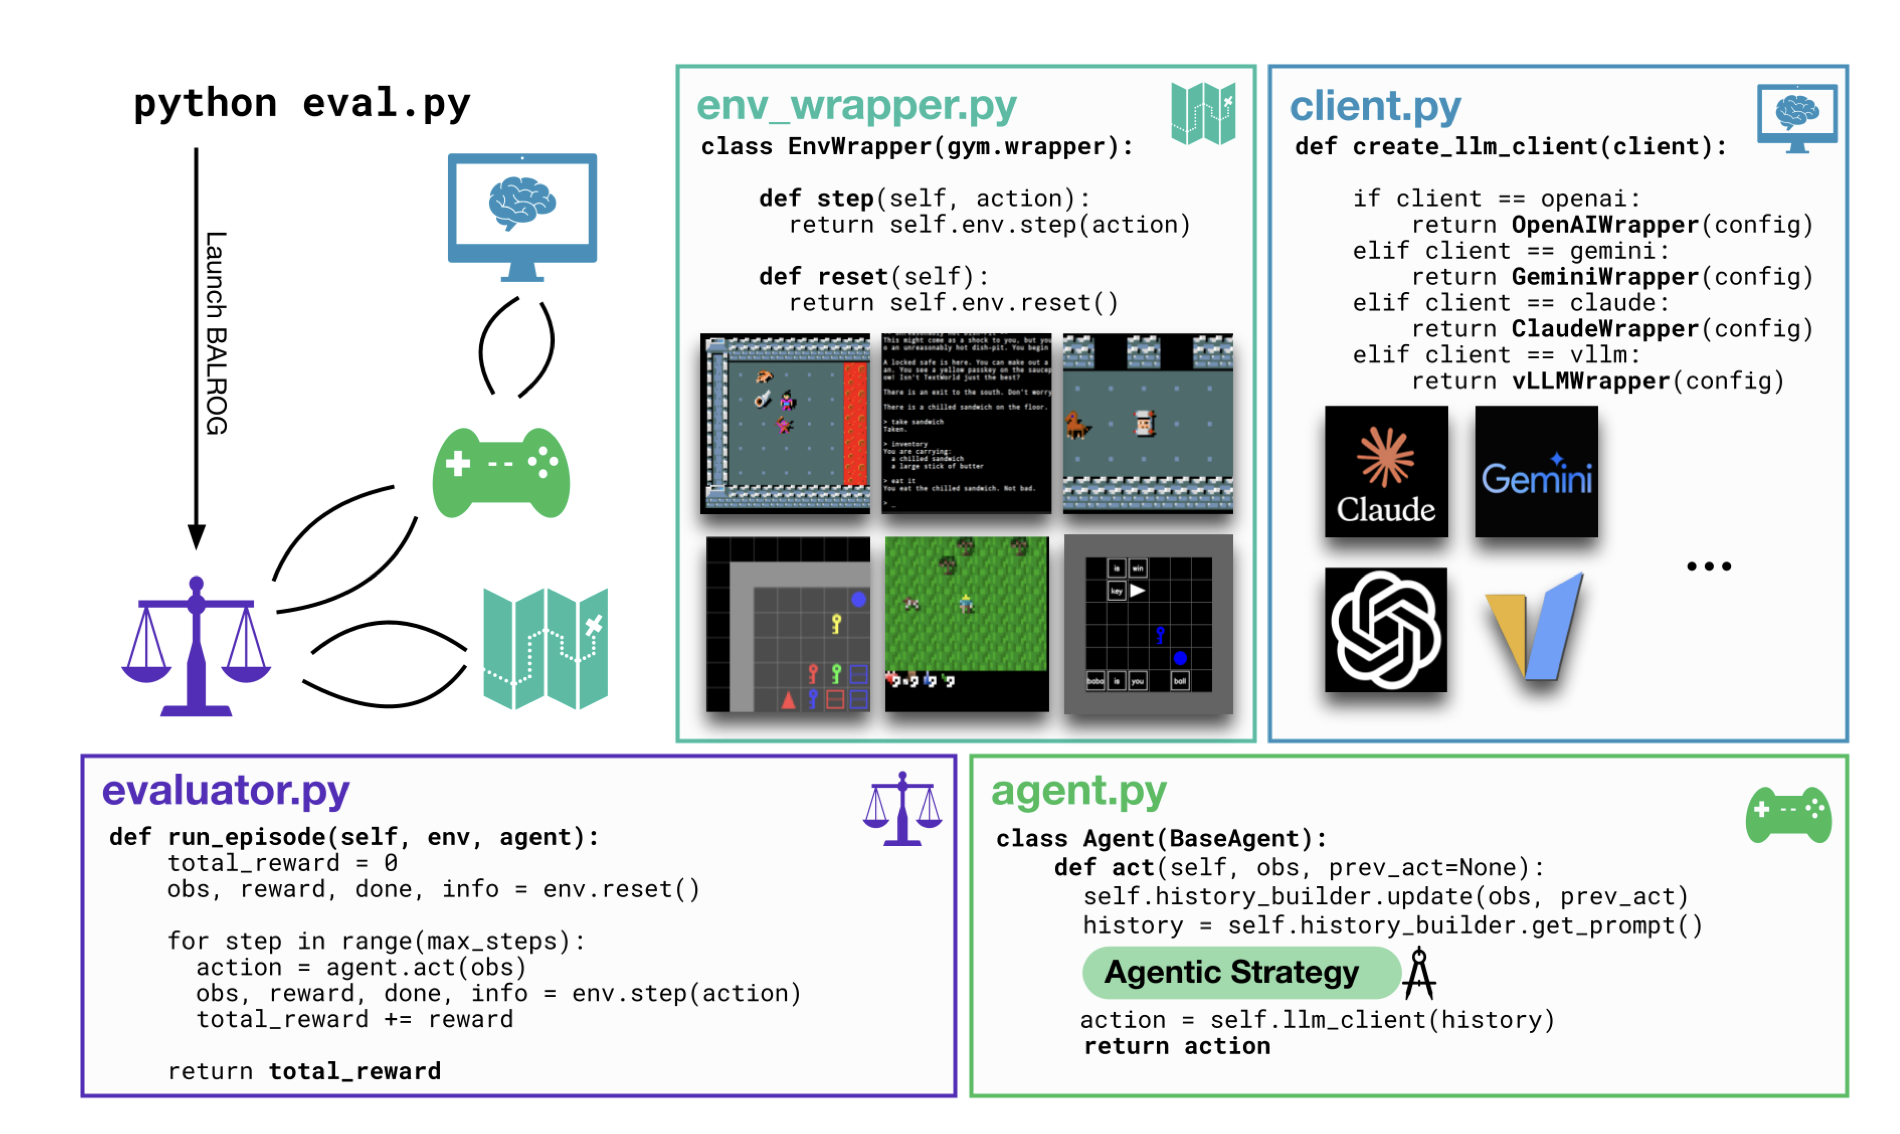
\includegraphics[width=\linewidth]{figures/balrogarch}};
\begin{scope}[x={(chTenArch.south east)},y={(chTenArch.north west)}]
\fill[white] (.107,.605) rectangle (.129,.802);
\node[rotate=-90,font=\small,inner sep=0] at (.115,.704) {启动 BALROG};
\fill[chTenStrategyBg] (.577,.128) rectangle (.724,.161);
\node[font=\bfseries\small,inner sep=0] at (.651,.144) {智能体策略};
\end{scope}
\end{tikzpicture}
\endgroup

    \caption{BALROG 的架构 \citep{paglieri2024balrog}。}
    \label{fig:balrogarch}
\end{figure}

\subsection{BALROG 架构}
现在，我们来看看 BALROG 框架的架构。图~\ref{fig:balrogarch}~展示了这一架构，图片取自论文 \citep{paglieri2024balrog}。

请熟悉 BALROG 系统。阅读论文 \citet{paglieri2024balrog}，你可以在 \url{https://arxiv.org/abs/2411.13543} 找到它，也可以访问 BALROG 网站 \url{https://balrogai.com}。

如果你还没有安装 BALROG，请使用 \verb|git clone| 命令将它安装到你的系统中。
访问 \url{https://balrogai.com}，或者直接前往 GitHub 代码仓库 \url{https://github.com/balrog-ai/BALROG}。将该仓库安装到你的本地计算机上。

决定你想使用哪个大语言模型。请注意，典型的 BALROG 智能体会在推进过程中的每一步调用大语言模型，因此调用次数很多。如果你想在本地运行大语言模型，请安装它，或者通过 Huggingface 使用它。如果你想使用基于云的（商业）大语言模型，请获取一个 API 密钥，并将它配置到你的环境中。如果服务提供免费的学生档位，你也可以考虑申请。使用前沿大语言模型的成本可能很高，但较旧、较小的模型通常便宜得多，其中一些仍然具有相当不错的能力。

BALROG 的 GitHub 仓库中的 README 提供了系统安装说明，以及如何为你选用的大语言模型配置 API 密钥，见代码~\ref{lst:key}。（在后面的一项练习中，我们将使用多个大语言模型，比较它们的性能。目前，我们只是尝试让系统运行起来，任何一个模型都可以。）
\begin{listing}
    \begin{minted}[
frame=lines,
framesep=2mm,
baselinestretch=1.0,
fontsize=\footnotesize,
linenos
]{bash}
        export OPENAI_API_KEY=<KEY>
        export ANTHROPIC_API_KEY=<KEY>
        export GEMINI_API_KEY=<KEY>
    \end{minted}
    \caption{配置 API 密钥。}\label{lst:key}
\end{listing}

\subsection{智能体}
请阅读 BALROG 的智能体教程：\url{https://github.com/balrog-ai/BALROG/blob/main/docs/agents.md}。在 BALROG 中，智能体是一小段 Python 代码，它用提示调用大语言模型，要求模型回答应当如何确定下一步。智能体代码负责接收来自模型的回答（观测），并选择下一个动作。大语言模型用于执行各种提示。

BALROG 遵循图~\ref{fig:rlD}~中的交互方式 D，即根据交互历史构造提示。

\subsubsection{提示构造器}
智能体根据先前的动作，也就是前几次交互中的观测／动作对，构造提示。
因此，用强化学习的术语来说，智能体承担策略的功能，根据传入的观测选择接下来执行的动作。

前往 \verb|prompt_builder| 目录，可以修改根据动作历史构造提示的方式。

\subsubsection{智能体}
智能体负责记忆功能：管理观测／动作历史。
智能体必须记录过去的观测与动作，以支持考虑上下文的决策。这一功能必须由我们在大语言模型之外实现。

BALROG 中的智能体代码会查询大语言模型：智能体向模型发送观测，接收响应，再利用这些响应决定在游戏中采取什么动作。

BALROG 提供了若干预先编写的智能体，你应当研究它们，以便设计自己的智能体。代码仓库包含一个朴素智能体和一个思维链智能体，还提供了能够更稳健地处理大语言模型响应的版本。

构建自己的智能体时，你很可能会以自定义智能体为基础。
BALROG 的智能体教程提供了一个简单规划智能体的示例。

\section{实现步骤}
下面，我们通过一些练习，帮助你探索如何构建自己的智能体。
\subsection{复现论文结果}

我们先尝试复现 BALROG 论文中的结果。
请查看 GitHub 上的 BALROG 代码：\url{https://github.com/balrog-ai/BALROG}。阅读评估指南、智能体开发教程，以及如何运行少样本学习实验，即上下文学习实验的说明。
在计算机上安装相关工具与正确版本的 Python，并将其加入 PATH。通过在命令提示符中启动 Python 解释器来检查版本：\verb|$ python|。

首先，运行标准评估，确认安装正确，见代码~\ref{lst:eval}。
\begin{listing}
    \begin{minted}[
frame=lines,
framesep=2mm,
baselinestretch=1.0,
fontsize=\footnotesize,
linenos
]{bash}
 python eval.py \
  agent.type=naive \
  agent.max_image_history=0 \
  agent.max_text_history=16 \
  eval.num_workers=16 \
  client.client_name=openai \
  client.model_id=gpt-4o-mini-2024-07-18       
    \end{minted}
    \caption{运行标准评估。}\label{lst:eval}
\end{listing}

\subsection{不同的大语言模型}

为了了解标准智能体采用不同大语言模型时，在各项基准测试中的表现，运行几个不同的大语言模型会很有帮助。
建议你都试一试闭源与开放的大语言模型，观察它们的表现。尤其是 OpenAI、Claude、DeepSeek、OLMo 和 Qwen 的开放版本，可能表现不错。

运行这些模型很重要，能够帮助你更深入地了解各个模型相对的优势。

\subsection{不同的谜题}
接下来，为了更好地理解基准测试，你应当在不同谜题问题中运行大语言模型智能体之后，仔细查看大语言模型的提示与回答。看看能否发现智能体在哪里失败、它的弱点在哪里。通过仔细检查每一个动作，并更深入地理解谜题，你也许能够想到改进智能体的方法。

\subsection{计算成本}
BALROG 智能体每走一步，都会调用一次大语言模型，而且提示往往很长。在这些谜题与游戏中，智能体需要走很多这样的步骤。用不同随机种子，在完整基准测试上运行不同的大语言模型，很容易就会消耗大量词元。

实验时，先尝试一个小而便宜的大语言模型，例如 Qwen-3B。从最简单的基准测试 BabyAI 和 Crafter 开始。如果你希望扩大实验范围，尽管尝试，但要留意计算成本。你希望获得洞见，也希望实验能够在合理时间内，以合理成本完成。

\subsection{实现自己的推理智能体}
现在，是实现你自己的学习智能体的时候了。
进入 balrog 的 agents 目录，编辑 \verb|custom.py| 文件。
代码~\ref{lst:agent}~重现了 BALROG README 中自定义智能体的代码。你可以使用代码~\ref{lst:agent-run}~中的命令运行它，该命令指定自定义智能体，并使用较少的 worker，以较低负载运行。当然，你也可以在命令中指定自己选用的大语言模型。

从提供的代码开始，运行它，了解它如何工作。然后，你可以尝试作一些小改进。试着修改给大语言模型的提示，以及 Python 代码处理智能体学习的方式；你可以修改历史提示构造器、计划，或者学习算法。

\begin{listing}
\setminted{breaklines,breakanywhere}
\begin{minted}[
frame=lines,
framesep=2mm,
baselinestretch=1.0,
fontsize=\footnotesize,
linenos
]{python}
from balrog.agents.base import BaseAgent
import re


class CustomAgent(BaseAgent):
    def __init__(self, client_factory, prompt_builder):
        super().__init__(client_factory, prompt_builder)
        self.client = client_factory()
        self.plan = None

    def act(self, obs, prev_action=None):
        if prev_action:
            self.prompt_builder.update_action(prev_action)
        self.prompt_builder.update_observation(obs)

        plan_text = f"Current Plan:\n{self.plan}\n" if self.plan else "You have no plan yet.\n"

        planning_instructions = """
Review the current plan above if present. Decide whether to continue with it or make changes.
If you make changes, provide the updated plan. Then, provide the next action to take. 
You must output an action at every step.
Format your answer in the following way:
PLAN: <your updated plan if changed, or "No changes to the plan." if the current plan is good>
ACTION: <your next action>
        """.strip()

        messages = self.prompt_builder.get_prompt()
        if messages and messages[-1].role == "user":
            messages[-1].content += "\n\n" + plan_text + "\n" + planning_instructions

        response = self.client.generate(messages)

        # Extract the plan and action from the LLM's response
        plan, action = self._extract_plan_and_action(response.completion)

        # Update the internal plan if it has changed
        if plan != "No changes to the plan.":
            self.plan = plan

        # Save the plan in the response.reasoning field and the action in response.completion
        response = response._replace(reasoning=plan, completion=action)
        return response

    def _extract_plan_and_action(self, response_text):
        plan_match = re.search(r"PLAN:\s*(.*?)(?=\nACTION:|\Z)", response_text, re.IGNORECASE | re.DOTALL)
        action_match = re.search(r"ACTION:\s*(.*)", response_text, re.IGNORECASE | re.DOTALL)

        plan = plan_match.group(1).strip() if plan_match else "No changes to the plan."
        action = action_match.group(1).strip() if action_match else None

        return plan, action
\end{minted}
    \caption{BALROG 中的智能体代码。}\label{lst:agent}
\end{listing}

\begin{listing}
    \begin{minted}[
frame=lines,
framesep=2mm,
baselinestretch=1.0,
fontsize=\footnotesize,
linenos
]{bash}
python eval.py \
  agent.type=custom \
  agent.max_image_history=0 \
  agent.max_history=16 \
  eval.num_workers=64 \
  client.client_name=openai \
  client.model_id=gpt-4o-mini-2024-07-18        
    \end{minted}
    \caption{运行智能体评估。}\label{lst:agent-run}
\end{listing}

\section{评估}
BALROG 会用进度百分比报告智能体的表现。记录你尝试的每项基准测试、每种智能体类型的进度数值。请用结构化的方式记录；你可以编写 Python 或 shell 脚本，自动运行实验并记录结果，也可以将进度绘成图表。可以考虑使用 wandb.ai。

哪些智能体类型表现良好？它们在哪些基准测试上表现良好？制作一个矩阵，记录你尝试的各类智能体在各类基准测试上的进度。

请注意，大语言模型实验在本质上具有非确定性：使用相同提示运行两次，可能得到不同结果。因此，每项实验都要运行多次。如果连续五次得到相同的结果，你就可以开始信任这些结果。如果结果差异很大，你可能需要调查原因。这是否纯粹是统计波动？降低温度能解决问题，还是另有原因？

不要盲目信任所报告的进度数值。你使用的是计算机上的代码，因此可能存在程序错误或其他问题。BALROG 系统便于你深入分析各次运行。它会将日志记录为 csv 文件，你可以用电子表格查看。检查其中一些运行，判断你看到的现象是否合理，或者智能体是否出现退化行为。如果出现了，就试着查明原因。你是否做错了什么？基准测试与智能体行为之间，是否存在意料之外的干扰？
奖励景观是否过于平坦，以致没有可供智能体追求的信号，它所做的只是在毫无意义地随机行动、原地打转？你能对此做些什么吗？

请注意，大语言模型领域，尤其是智能体大语言模型领域，还很年轻，我们的认识与软件框架都尚未稳定下来。出现一些意料之外的结果是正常的，你也可能遇到一些挑战或挫折。

结构化的实验方式与结果记录方式，会成为你的好帮手。通过规划与组织，运行、评估和改进实际的智能体大语言模型实验，可以成为一项令人愉快的练习。

\section{自我反思}
当你已经能够复现基准测试结果，也对智能体进行了一些实验之后，也许会想尝试更大的挑战。本节中，我们将尝试为 BALROG 智能体扩展自我反思能力，让大语言模型承担不同角色，例如评估与动作选择。自我反思和任何追逐一个本身也在被优化的目标的自适应系统一样，可能容易出现不稳定与振荡。因此，在尝试自我反思的想法之前，上一小节中的基础学习器系统必须能够正常工作，并以稳定、可预测的方式收敛。
请回到前面那一节，确认一切都能按照你的预期运行。

近期有许多工作尝试改进大语言模型智能体。我们在此介绍两项：ReAct \citep{yao2022react} 与 Reflexion \citep{shinn2024reflexion}。ReAct 主要关注提示，而 Reflexion 则引入了新的智能体算法，包括短期记忆与长期记忆。

\begin{figure}
    \centering
    % 依照 figures/react.png 重排完整问答、推理、动作与观测；原错误答案及工具调用保留。
\begingroup
\footnotesize
\linespread{1.05}\selectfont
\tcbset{chTenPanel/.style={enhanced,colback=white,colframe=black!45,boxrule=.4pt,arc=1mm,
  left=4pt,right=4pt,top=4pt,bottom=4pt,boxsep=0pt,before skip=0pt,after skip=5pt,
  colbacktitle=black!6,coltitle=black,fonttitle=\bfseries\small,center title,before upper={\raggedright}}}
\newcommand{\chTenBad}{\hfill\textcolor{red!65}{\large$\times$}}
\newcommand{\chTenGood}{\hfill\tikz[baseline=-.4ex,x=1ex,y=1ex]{\draw[green!50!black,line width=1.2pt,line cap=round,line join=round] (0,.4)--(.35,0)--(1.1,1);}}
\newcommand{\chTenTool}[1]{\textcolor{blue!65!black}{\texttt{#1}}}
\begin{minipage}[t]{.485\linewidth}
\vspace{0pt}
\raggedright
\begin{tcolorbox}[chTenPanel]
\textbf{问题：}除了 Apple Remote，还有什么设备可以控制 Apple Remote 最初设计用来与之交互的程序？
\end{tcolorbox}
\begin{tcolorbox}[chTenPanel,title=标准方式]
\textbf{答案：}\texttt{iPod}\chTenBad
\end{tcolorbox}
\begin{tcolorbox}[chTenPanel,title=仅推理]
\textbf{思考：}让我们逐步思考。\par
\colorbox{red!20}{\parbox{\dimexpr\linewidth-2\fboxsep\relax}{Apple Remote 最初设计用来与 Apple TV 交互。Apple TV 可以由 iPhone、iPad 和 iPod Touch 控制。}}
\par\noindent 因此，答案是 iPhone、iPad 和 iPod Touch。

\smallskip
\textbf{答案：}\texttt{iPhone, iPad, iPod Touch}\chTenBad
\end{tcolorbox}
\begin{tcolorbox}[chTenPanel,title=仅行动]
\textbf{动作 1：}\chTenTool{Search[Apple Remote]}\\
\textbf{观测 1：}Apple Remote 是一种遥控器，推出于……\\
\textbf{动作 2：}\chTenTool{Search[Front Row]}\\
\textbf{观测 2：}未找到 [Front Row]。相近结果：……\\
\textbf{动作 3：}\chTenTool{Search[Front Row (software)]}\\
\textbf{观测 3：}Front Row 是一款已停止开发的媒体软件……\\
\textbf{动作 4：}\chTenTool{Finish[}\colorbox{red!20}{\texttt{yes}}\chTenTool{]}\chTenBad
\end{tcolorbox}
\end{minipage}\hfill
\begin{minipage}[t]{.485\linewidth}
\vspace{0pt}
\raggedright
\begin{tcolorbox}[chTenPanel,title=ReAct]
\textbf{思考 1：}我需要搜索 Apple Remote，并找到它最初设计用来与之交互的程序。\\
\textbf{动作 1：}\chTenTool{Search[Apple Remote]}\\
\textbf{观测 1：}Apple Remote 是 Apple 于 2005 年 10 月推出的一种遥控器……最初设计用来控制\colorbox{green!25}{Front Row 媒体中心}程序……

\smallskip
\textbf{思考 2：}Apple Remote 最初设计用来控制 Front Row 媒体中心程序。我接下来需要搜索 Front Row，找出还有什么设备可以控制它。\\
\textbf{动作 2：}\chTenTool{Search[Front Row]}\\
\textbf{观测 2：}未找到 [Front Row]。相近结果：['Front Row Seat to Earth', 'Front Row Motorsports', '\textcolor{green!35!black}{Front Row (software)}', …]

\smallskip
\textbf{思考 3：}未找到 Front Row。我需要搜索\textcolor{green!35!black}{Front Row (software)}。\\
\textbf{动作 3：}\chTenTool{Search[Front Row (software)]}\\
\textbf{观测 3：}Front Row 是一款已停止开发的媒体中心软件……

\smallskip
\textbf{思考 4：}\par
\noindent\colorbox{green!25}{\parbox{\dimexpr\linewidth-2\fboxsep\relax}{Front Row (software) 可由 Apple Remote 或键盘功能键控制。}}\par
\noindent 因此，答案是键盘功能键。\\
\textbf{动作 4：}\chTenTool{Finish[keyboard function keys]}\chTenGood
\end{tcolorbox}
\end{minipage}
\endgroup

    \caption{ReAct 执行搜索的示例 \citep{yao2022react}。}
    \label{fig:react}
\end{figure}

\paragraph{ReAct}
ReAct 使用提示与世界交互。ReAct 提倡使用工具查找信息，见图~\ref{fig:react}。ReAct 的原始网站是 \url{https://react-lm.github.io}，代码仓库位于 \url{https://github.com/ysymyth/ReAct}。LangChain\footnote{见 \url{https://docs.langchain.com/oss/python/langchain/overview}。}与 BeeAI\footnote{见 \url{https://github.com/i-am-bee/beeai-framework/blob/main/python/examples/agents/react.py}。}框架也实现了 ReAct 提示方法。

请查看这些框架，理解 ReAct 引入的基于提示的智能体交互方式。然后，在 BALROG 中实现这种基于提示的交互。它是否改善了性能？对于哪些游戏，查找外部信息会有帮助？对于哪些游戏则没有帮助？

\paragraph{Reflexion}
ReAct 基于提示，允许交互式查找；Reflexion 方法则引入了用 Python 编写的智能体，允许实现更复杂的智能体行为。
Reflexion 在不同上下文中，以不同提示使用同一个大语言模型。
它的基本假设是，批评现有提示有什么问题，比从头提出一个有效的提示更容易。

Reflexion 是一种流行的自我反思架构 \citep{shinn2024reflexion}。Reflexion 的主页是 \url{https://github.com/noahshinn/reflexion}。介绍其主要思想的一篇博客文章位于：\url{https://nanothoughts.substack.com/p/reflecting-on-reflexion}。

\begin{figure}
    \centering
    % 依照 figures/reflexion3.png 重绘，全部外部/内部反馈、轨迹、经验和动作连线对应原图。
\resizebox{.9\linewidth}{!}{%
\begin{tikzpicture}[x=1cm,y=1cm,
 every node/.style={font=\normalsize,align=center,inner sep=4pt},
 lm/.style={draw=black!60,fill=cyan!8!gray!15,rounded corners=1.5mm,line width=.8pt,minimum width=4.5cm,minimum height=.85cm},
 memory/.style={draw=black!60,fill=yellow!15,line width=.8pt,minimum width=4.4cm,minimum height=1.2cm},
 flow/.style={-{Stealth[length=2.5mm,width=1.8mm]},draw=black!60,line width=.9pt},
 label/.style={font=\small,fill=black!2,inner sep=2pt}]
\filldraw[draw=black!60,fill=black!2,line width=.8pt] (.6,2.5) rectangle (12.8,10.2);
\node[font=\bfseries\Large] at (6.7,9.55) {智能体};
\node[lm] (reflect) at (7.0,8.2) {自我反思（LM）};
\node[lm] (eval) at (3.7,6.25) {评估者（LM）};
\node[memory] (traj) at (3.7,4.0) {轨迹\\（短期记忆）};
\node[memory] (experience) at (9.7,6.0) {经验\\（长期记忆）};
\node[lm] (actor) at (9.7,4.0) {行动者（LM）};
\node[draw=black!60,fill=black!7,line width=.8pt,minimum width=4.5cm,minimum height=.9cm,font=\bfseries\large] (env) at (6.4,.7) {环境};

\draw[flow] (traj.north) -- (eval.south);
\draw[flow] (traj.east) -- (actor.west);
\draw[flow] (experience.south) -- (actor.north);
\draw[flow] (reflect.east) -- (10.3,8.2) -- (10.3,6.6);
\node[label] at (11.25,7.35) {反思文本};
\draw[draw=black!60,line width=.9pt] (eval.north) -- (3.7,8.2);
\node[label] at (2.65,7.35) {内部\\反馈};
\draw[flow] (env.west) -- (0,.7) -- (0,8.2) -- (reflect.west);
\node[label] at (2.65,8.65) {外部反馈};
\draw[flow] (0,4.0) -- (traj.west);
\node[font=\normalsize,fill=white,inner sep=4pt] at (2.1,.7) {观测／奖励};
\draw[flow] (actor.east) -- (13.3,4.0) -- (13.3,.7) -- (env.east);
\node[font=\normalsize,fill=white,inner sep=4pt] at (10.8,.7) {动作};
\end{tikzpicture}%
}

    \caption{Reflexion 架构 \citep{shinn2024reflexion}。}
    \label{fig:reflexion-alg}
\end{figure}

\begin{figure}
    \centering
    % 依照 figures/reflexion-code.png 重排。while 的原条件为 or，按原文保留。
\begingroup
\small
\renewcommand{\arraystretch}{1.25}
\begin{minipage}{.94\linewidth}
\begin{tabularx}{\linewidth}{@{}X@{}}
\toprule
\textbf{算法 1}\quad 通过自我反思进行强化 \\
\midrule
初始化行动者、评估者与自我反思模型：$M_a,M_e,M_{sr}$ \\
初始化策略 $\pi_\theta(a_i\mid s_i)$，$\theta=\{M_a,mem\}$ \\
使用 $\pi_\theta$ 生成初始轨迹 \\
使用 $M_e$ 评估 $\tau_0$ \\
使用 $M_{sr}$ 生成初始自我反思 $sr_0$ \\
设置 $mem\leftarrow[sr_0]$ \\
设置 $t=0$ \\
\textbf{当} $M_e$ 未通过 \textbf{或} $t<\text{max trials}$ \textbf{执行} \\
\hspace*{1.5em}使用 $\pi_\theta$ 生成 $\tau_t=[a_0,o_0,\ldots a_i,o_i]$ \\
\hspace*{1.5em}使用 $M_e$ 评估 $\tau_t$ \\
\hspace*{1.5em}使用 $M_{sr}$ 生成自我反思 $sr_t$ \\
\hspace*{1.5em}将 $sr_t$ 追加至 $mem$ \\
\hspace*{1.5em}递增 $t$ \\
\textbf{结束循环} \\
\textbf{返回} \\
\bottomrule
\end{tabularx}
\end{minipage}
\endgroup

    \caption{Reflexion 算法 \citep{shinn2024reflexion}。}
    \label{fig:reflexion-code}
\end{figure}

图~\ref{fig:reflexion-alg}~展示了 Reflexion 的一般概念、不同的提示，以及不同类型的记忆。图~\ref{fig:reflexion-code}~展示了 Reflexion 的代码，其中第 3、5、6 行分别调用大语言模型（$M_a$、$M_e$ 与 $M_{sr}$），第 9、11、12 行也包含这些调用。请注意，这是一段伪代码，记忆管理、提示管理与收敛判据等重要细节都尚未明确。
请查看 GitHub 仓库，了解细节。

Reflexion 对同一个大语言模型使用不同提示，这可能导致学习不稳定与循环。此外，它的记忆管理相对简单，可能超出上下文长度限制。一个思路是实现分块或其他记忆压缩方法，可以手动用 Python 实现，也可以使用大语言模型。

首先试用 Reflexion 代码仓库，尝试让它在 Reflexion 的应用中运行起来，例如 AlfWorld 和 HotpotQA。

\paragraph{扩展}
现在，尝试在 BALROG 中实现一个 Reflexion 智能体，并在 BALROG 基准测试上运行。
你遇到了什么问题？与标准 BALROG 智能体相比，Reflexion 是否提升了性能？

接下来，进一步拓展这个问题。你可以尝试从文献中寻找其他反思方法，也可以尝试自己创造新的反思方法。你可以尝试不同类型的应用，考察自己的方法表现如何。当然，你也可以尝试其他大语言模型。

\section{结语}
本章通过一个实践案例研究，考察了大语言模型如何进行自我反思。我们使用了 BALROG，一个流行的推理任务基准测试套件。BALROG 混合了从简单到困难的游戏，其中一些游戏对大语言模型而言很难玩好。
BALROG 套件采用开放式设计。我们可以编写自己的智能体代码，随后在 BALROG 的游戏中运行。

这是一次重要的实践案例研究。
你已经探索了如何为上下文推理编写自己的智能体代码。通过实现自我反思，你也超越了基础学习。你已经在不同的大语言模型上，利用极具挑战性的基准测试，探索了自我反思的稳定性。

\bibliographystyle{plainnat}
\bibliography{agenticbook,refs,case,synthetic}
